% Options for packages loaded elsewhere
% Options for packages loaded elsewhere
\PassOptionsToPackage{unicode}{hyperref}
\PassOptionsToPackage{hyphens}{url}
\PassOptionsToPackage{dvipsnames,svgnames,x11names}{xcolor}
%
\documentclass[
  letterpaper,
  DIV=11,
  numbers=noendperiod]{scrartcl}
\usepackage{xcolor}
\usepackage{amsmath,amssymb}
\setcounter{secnumdepth}{-\maxdimen} % remove section numbering
\usepackage{iftex}
\ifPDFTeX
  \usepackage[T1]{fontenc}
  \usepackage[utf8]{inputenc}
  \usepackage{textcomp} % provide euro and other symbols
\else % if luatex or xetex
  \usepackage{unicode-math} % this also loads fontspec
  \defaultfontfeatures{Scale=MatchLowercase}
  \defaultfontfeatures[\rmfamily]{Ligatures=TeX,Scale=1}
\fi
\usepackage{lmodern}
\ifPDFTeX\else
  % xetex/luatex font selection
\fi
% Use upquote if available, for straight quotes in verbatim environments
\IfFileExists{upquote.sty}{\usepackage{upquote}}{}
\IfFileExists{microtype.sty}{% use microtype if available
  \usepackage[]{microtype}
  \UseMicrotypeSet[protrusion]{basicmath} % disable protrusion for tt fonts
}{}
\makeatletter
\@ifundefined{KOMAClassName}{% if non-KOMA class
  \IfFileExists{parskip.sty}{%
    \usepackage{parskip}
  }{% else
    \setlength{\parindent}{0pt}
    \setlength{\parskip}{6pt plus 2pt minus 1pt}}
}{% if KOMA class
  \KOMAoptions{parskip=half}}
\makeatother
% Make \paragraph and \subparagraph free-standing
\makeatletter
\ifx\paragraph\undefined\else
  \let\oldparagraph\paragraph
  \renewcommand{\paragraph}{
    \@ifstar
      \xxxParagraphStar
      \xxxParagraphNoStar
  }
  \newcommand{\xxxParagraphStar}[1]{\oldparagraph*{#1}\mbox{}}
  \newcommand{\xxxParagraphNoStar}[1]{\oldparagraph{#1}\mbox{}}
\fi
\ifx\subparagraph\undefined\else
  \let\oldsubparagraph\subparagraph
  \renewcommand{\subparagraph}{
    \@ifstar
      \xxxSubParagraphStar
      \xxxSubParagraphNoStar
  }
  \newcommand{\xxxSubParagraphStar}[1]{\oldsubparagraph*{#1}\mbox{}}
  \newcommand{\xxxSubParagraphNoStar}[1]{\oldsubparagraph{#1}\mbox{}}
\fi
\makeatother

\usepackage{color}
\usepackage{fancyvrb}
\newcommand{\VerbBar}{|}
\newcommand{\VERB}{\Verb[commandchars=\\\{\}]}
\DefineVerbatimEnvironment{Highlighting}{Verbatim}{commandchars=\\\{\}}
% Add ',fontsize=\small' for more characters per line
\usepackage{framed}
\definecolor{shadecolor}{RGB}{241,243,245}
\newenvironment{Shaded}{\begin{snugshade}}{\end{snugshade}}
\newcommand{\AlertTok}[1]{\textcolor[rgb]{0.68,0.00,0.00}{#1}}
\newcommand{\AnnotationTok}[1]{\textcolor[rgb]{0.37,0.37,0.37}{#1}}
\newcommand{\AttributeTok}[1]{\textcolor[rgb]{0.40,0.45,0.13}{#1}}
\newcommand{\BaseNTok}[1]{\textcolor[rgb]{0.68,0.00,0.00}{#1}}
\newcommand{\BuiltInTok}[1]{\textcolor[rgb]{0.00,0.23,0.31}{#1}}
\newcommand{\CharTok}[1]{\textcolor[rgb]{0.13,0.47,0.30}{#1}}
\newcommand{\CommentTok}[1]{\textcolor[rgb]{0.37,0.37,0.37}{#1}}
\newcommand{\CommentVarTok}[1]{\textcolor[rgb]{0.37,0.37,0.37}{\textit{#1}}}
\newcommand{\ConstantTok}[1]{\textcolor[rgb]{0.56,0.35,0.01}{#1}}
\newcommand{\ControlFlowTok}[1]{\textcolor[rgb]{0.00,0.23,0.31}{\textbf{#1}}}
\newcommand{\DataTypeTok}[1]{\textcolor[rgb]{0.68,0.00,0.00}{#1}}
\newcommand{\DecValTok}[1]{\textcolor[rgb]{0.68,0.00,0.00}{#1}}
\newcommand{\DocumentationTok}[1]{\textcolor[rgb]{0.37,0.37,0.37}{\textit{#1}}}
\newcommand{\ErrorTok}[1]{\textcolor[rgb]{0.68,0.00,0.00}{#1}}
\newcommand{\ExtensionTok}[1]{\textcolor[rgb]{0.00,0.23,0.31}{#1}}
\newcommand{\FloatTok}[1]{\textcolor[rgb]{0.68,0.00,0.00}{#1}}
\newcommand{\FunctionTok}[1]{\textcolor[rgb]{0.28,0.35,0.67}{#1}}
\newcommand{\ImportTok}[1]{\textcolor[rgb]{0.00,0.46,0.62}{#1}}
\newcommand{\InformationTok}[1]{\textcolor[rgb]{0.37,0.37,0.37}{#1}}
\newcommand{\KeywordTok}[1]{\textcolor[rgb]{0.00,0.23,0.31}{\textbf{#1}}}
\newcommand{\NormalTok}[1]{\textcolor[rgb]{0.00,0.23,0.31}{#1}}
\newcommand{\OperatorTok}[1]{\textcolor[rgb]{0.37,0.37,0.37}{#1}}
\newcommand{\OtherTok}[1]{\textcolor[rgb]{0.00,0.23,0.31}{#1}}
\newcommand{\PreprocessorTok}[1]{\textcolor[rgb]{0.68,0.00,0.00}{#1}}
\newcommand{\RegionMarkerTok}[1]{\textcolor[rgb]{0.00,0.23,0.31}{#1}}
\newcommand{\SpecialCharTok}[1]{\textcolor[rgb]{0.37,0.37,0.37}{#1}}
\newcommand{\SpecialStringTok}[1]{\textcolor[rgb]{0.13,0.47,0.30}{#1}}
\newcommand{\StringTok}[1]{\textcolor[rgb]{0.13,0.47,0.30}{#1}}
\newcommand{\VariableTok}[1]{\textcolor[rgb]{0.07,0.07,0.07}{#1}}
\newcommand{\VerbatimStringTok}[1]{\textcolor[rgb]{0.13,0.47,0.30}{#1}}
\newcommand{\WarningTok}[1]{\textcolor[rgb]{0.37,0.37,0.37}{\textit{#1}}}

\usepackage{longtable,booktabs,array}
\usepackage{calc} % for calculating minipage widths
% Correct order of tables after \paragraph or \subparagraph
\usepackage{etoolbox}
\makeatletter
\patchcmd\longtable{\par}{\if@noskipsec\mbox{}\fi\par}{}{}
\makeatother
% Allow footnotes in longtable head/foot
\IfFileExists{footnotehyper.sty}{\usepackage{footnotehyper}}{\usepackage{footnote}}
\makesavenoteenv{longtable}
\usepackage{graphicx}
\makeatletter
\newsavebox\pandoc@box
\newcommand*\pandocbounded[1]{% scales image to fit in text height/width
  \sbox\pandoc@box{#1}%
  \Gscale@div\@tempa{\textheight}{\dimexpr\ht\pandoc@box+\dp\pandoc@box\relax}%
  \Gscale@div\@tempb{\linewidth}{\wd\pandoc@box}%
  \ifdim\@tempb\p@<\@tempa\p@\let\@tempa\@tempb\fi% select the smaller of both
  \ifdim\@tempa\p@<\p@\scalebox{\@tempa}{\usebox\pandoc@box}%
  \else\usebox{\pandoc@box}%
  \fi%
}
% Set default figure placement to htbp
\def\fps@figure{htbp}
\makeatother





\setlength{\emergencystretch}{3em} % prevent overfull lines

\providecommand{\tightlist}{%
  \setlength{\itemsep}{0pt}\setlength{\parskip}{0pt}}



 


\KOMAoption{captions}{tableheading}
\makeatletter
\@ifpackageloaded{caption}{}{\usepackage{caption}}
\AtBeginDocument{%
\ifdefined\contentsname
  \renewcommand*\contentsname{Table of contents}
\else
  \newcommand\contentsname{Table of contents}
\fi
\ifdefined\listfigurename
  \renewcommand*\listfigurename{List of Figures}
\else
  \newcommand\listfigurename{List of Figures}
\fi
\ifdefined\listtablename
  \renewcommand*\listtablename{List of Tables}
\else
  \newcommand\listtablename{List of Tables}
\fi
\ifdefined\figurename
  \renewcommand*\figurename{Figure}
\else
  \newcommand\figurename{Figure}
\fi
\ifdefined\tablename
  \renewcommand*\tablename{Table}
\else
  \newcommand\tablename{Table}
\fi
}
\@ifpackageloaded{float}{}{\usepackage{float}}
\floatstyle{ruled}
\@ifundefined{c@chapter}{\newfloat{codelisting}{h}{lop}}{\newfloat{codelisting}{h}{lop}[chapter]}
\floatname{codelisting}{Listing}
\newcommand*\listoflistings{\listof{codelisting}{List of Listings}}
\makeatother
\makeatletter
\makeatother
\makeatletter
\@ifpackageloaded{caption}{}{\usepackage{caption}}
\@ifpackageloaded{subcaption}{}{\usepackage{subcaption}}
\makeatother
\usepackage{bookmark}
\IfFileExists{xurl.sty}{\usepackage{xurl}}{} % add URL line breaks if available
\urlstyle{same}
\hypersetup{
  pdftitle={homework-03},
  pdfauthor={Iris Carnahan},
  colorlinks=true,
  linkcolor={blue},
  filecolor={Maroon},
  citecolor={Blue},
  urlcolor={Blue},
  pdfcreator={LaTeX via pandoc}}


\title{homework-03}
\author{Iris Carnahan}
\date{2026-05-24}
\begin{document}
\maketitle


\section{Set-Up Tasks}\label{set-up-tasks}

\begin{Shaded}
\begin{Highlighting}[]
\FunctionTok{library}\NormalTok{(tidyverse) }\CommentTok{\# general use}
\FunctionTok{library}\NormalTok{(here) }\CommentTok{\# cleaning data frames}
\FunctionTok{library}\NormalTok{(janitor) }\CommentTok{\# file/folder organization}
\FunctionTok{library}\NormalTok{(readxl) }\CommentTok{\# reading .xlsx files}
\FunctionTok{library}\NormalTok{(ggeffects) }\CommentTok{\# calculating the data}
\CommentTok{\# reading in \textasciigrave{}temp{-}kelp\textasciigrave{} csv file}
\NormalTok{temp\_kelp }\OtherTok{\textless{}{-}} \FunctionTok{read.csv}\NormalTok{(}
  \FunctionTok{here}\NormalTok{(}\StringTok{"data"}\NormalTok{, }\StringTok{"temp{-}kelp.csv"}\NormalTok{)}
\NormalTok{)}
\CommentTok{\# reading in \textasciigrave{}personal\_data\_wk8\textasciigrave{} csv file}
\NormalTok{my\_data }\OtherTok{\textless{}{-}} \FunctionTok{read.csv}\NormalTok{(}
  \FunctionTok{here}\NormalTok{(}\StringTok{"data"}\NormalTok{, }\StringTok{"my\_es\_data.csv"}\NormalTok{)}
\NormalTok{)}
\CommentTok{\# reading in \textasciigrave{}bike\_to\_class\textasciigrave{} csv file}
\NormalTok{bike\_to\_class }\OtherTok{\textless{}{-}} \FunctionTok{read.csv}\NormalTok{(}
  \FunctionTok{here}\NormalTok{(}\StringTok{"data"}\NormalTok{, }\StringTok{"bike\_to\_class.csv"}\NormalTok{)}
\NormalTok{)}
\end{Highlighting}
\end{Shaded}

\section{Problem 1}\label{problem-1}

\subsection{a. Appropriate test}\label{a.-appropriate-test}

To determine the strength of the relationship between these variables, a
Pearson's or Spearman rank correlation can be used. Pearson's
correlations measure the direction of a linear relationship with
continuous variables, while a Spearman rank correlation measures
monotonic relationships between any variables (can be ordinal or
continuous).

\subsection{b. Visualization}\label{b.-visualization}

\begin{Shaded}
\begin{Highlighting}[]
\CommentTok{\# base layer: ggplot using \textasciigrave{}temp\_kelp\textasciigrave{}}
\FunctionTok{ggplot}\NormalTok{(}\AttributeTok{data =}\NormalTok{ temp\_kelp,}
       \CommentTok{\# x{-}axis: temperature in Celsius}
       \CommentTok{\# y{-}axis: kelp elongation rate (cm/day)}
       \AttributeTok{mapping =} \FunctionTok{aes}\NormalTok{(}\AttributeTok{x =}\NormalTok{ temp\_c,}
                     \AttributeTok{y =}\NormalTok{ kelp\_elong)) }\SpecialCharTok{+}
  \CommentTok{\# first layer: geom point to represent individual observations}
  \CommentTok{\# changing color from default to \textasciigrave{}red\textasciigrave{}}
  \FunctionTok{geom\_point}\NormalTok{(}\AttributeTok{color =} \StringTok{"red"}\NormalTok{) }\SpecialCharTok{+}
  \CommentTok{\# relabeling x{-} and y{-}axes, adding a title}
  \FunctionTok{labs}\NormalTok{(}\AttributeTok{x =} \StringTok{"Kelp Elongation Rate (cm/day)"}\NormalTok{,}
       \AttributeTok{y =} \StringTok{"Temperature (\textbackslash{}u00B0C)"}\NormalTok{) }\SpecialCharTok{+}
  \CommentTok{\# changing theme}
  \FunctionTok{theme\_minimal}\NormalTok{()}
\end{Highlighting}
\end{Shaded}

\pandocbounded{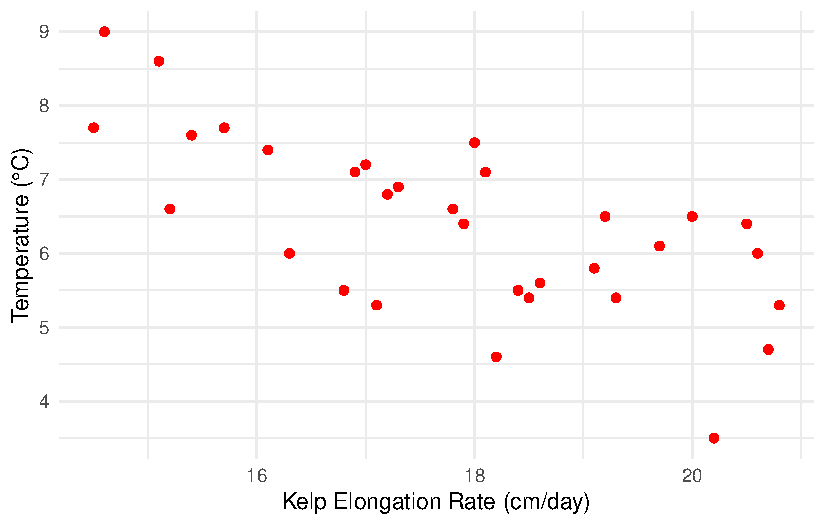
\includegraphics[keepaspectratio]{homework-03_files/figure-pdf/correlation-visualization-1.pdf}}

\subsection{c.~Assumption checks}\label{c.-assumption-checks}

\subsubsection{Check assumptions}\label{check-assumptions}

\begin{Shaded}
\begin{Highlighting}[]
\CommentTok{\# base layer: ggplot}
\FunctionTok{ggplot}\NormalTok{(}\AttributeTok{data =}\NormalTok{ temp\_kelp, }\CommentTok{\# starting data frame}
\FunctionTok{aes}\NormalTok{(}\AttributeTok{sample =}\NormalTok{ kelp\_elong)) }\SpecialCharTok{+} \CommentTok{\# y{-}axis for QQ plot}
\CommentTok{\# first layer: QQ reference line}
\FunctionTok{geom\_qq\_line}\NormalTok{(}\AttributeTok{color =} \StringTok{"red"}\NormalTok{) }\SpecialCharTok{+} \CommentTok{\# adding a color}
\CommentTok{\# second layer: QQ plot}
\FunctionTok{geom\_qq}\NormalTok{()}
\end{Highlighting}
\end{Shaded}

\pandocbounded{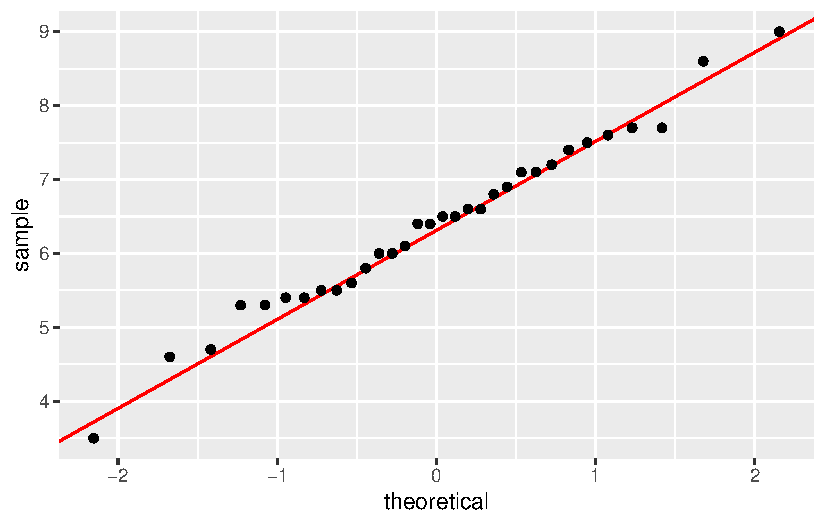
\includegraphics[keepaspectratio]{homework-03_files/figure-pdf/QQ-plot-normality-1.pdf}}

\begin{Shaded}
\begin{Highlighting}[]
\CommentTok{\# base layer: ggplot using \textasciigrave{}temp\_kelp\textasciigrave{}}
\FunctionTok{ggplot}\NormalTok{(}\AttributeTok{data =}\NormalTok{ temp\_kelp,}
       \CommentTok{\# x{-}axis: temperature in Celsius}
       \CommentTok{\# y{-}axis: kelp elongation rate (cm/day)}
       \AttributeTok{mapping =} \FunctionTok{aes}\NormalTok{(}\AttributeTok{x =}\NormalTok{ temp\_c,}
                     \AttributeTok{y =}\NormalTok{ kelp\_elong)) }\SpecialCharTok{+}
  \CommentTok{\# first layer: geom point to represent individual observations}
  \CommentTok{\# changing color from default to \textasciigrave{}red\textasciigrave{}}
  \FunctionTok{geom\_point}\NormalTok{(}\AttributeTok{color =} \StringTok{"red"}\NormalTok{) }\SpecialCharTok{+}
  \CommentTok{\# relabeling x{-} and y{-}axes, adding a title}
  \FunctionTok{labs}\NormalTok{(}\AttributeTok{x =} \StringTok{"Kelp Elongation Rate (cm/day)"}\NormalTok{,}
       \AttributeTok{y =} \StringTok{"Temperature (\textbackslash{}u00B0C)"}\NormalTok{) }\SpecialCharTok{+}
  \CommentTok{\# changing theme}
  \FunctionTok{theme\_minimal}\NormalTok{()}
\end{Highlighting}
\end{Shaded}

\pandocbounded{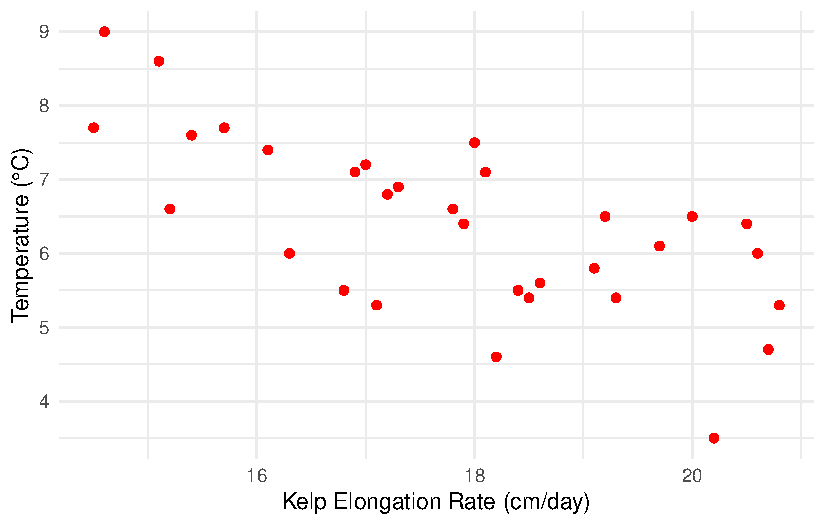
\includegraphics[keepaspectratio]{homework-03_files/figure-pdf/linearity-check-1.pdf}}

\begin{Shaded}
\begin{Highlighting}[]
\CommentTok{\# creating model called \textasciigrave{}assump\_check\textasciigrave{}}
\CommentTok{\# formula: change is kelp elongation rate as a function of temperature}
\NormalTok{assump\_check }\OtherTok{\textless{}{-}} \FunctionTok{lm}\NormalTok{(kelp\_elong }\SpecialCharTok{\textasciitilde{}}\NormalTok{ temp\_c, }\AttributeTok{data =}\NormalTok{ temp\_kelp)  }\CommentTok{\# data frame: \textasciigrave{}temp\_kelp\textasciigrave{}}
\CommentTok{\# displaying residual vs. fitted plot only}
\FunctionTok{plot}\NormalTok{(assump\_check, }\AttributeTok{which =} \DecValTok{5}\NormalTok{)}
\end{Highlighting}
\end{Shaded}

\pandocbounded{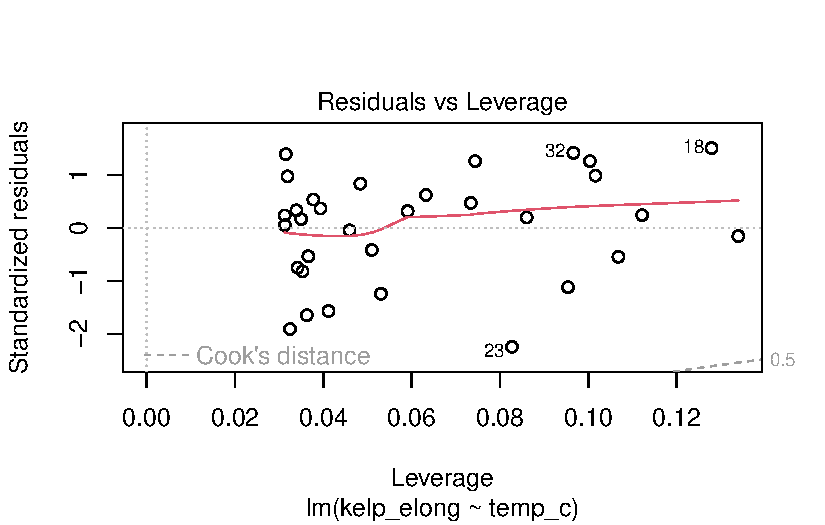
\includegraphics[keepaspectratio]{homework-03_files/figure-pdf/residual-vs-leverage-plot-1.pdf}}

I checked the assumptions of linearity using a scatter plot, that no
major outliers are affecting that line using a residuals vs.~leverage
plot, and for normality using a Q-Q plot. Given each plot, I would say
that this relationship is close enough to be considered normal
considering the minor deviations from the theoretical distribution,
there is a mostly linear relationship shown by the general downward
pattern of the scatterplot and assumed normality, and the residuals are
within the Cook's distance lines, so there are no major outliers
influencing the model.

\subsubsection{Run test}\label{run-test}

\begin{Shaded}
\begin{Highlighting}[]
\CommentTok{\# displaying assumption check to generate outputs}
\FunctionTok{summary}\NormalTok{(assump\_check)}
\end{Highlighting}
\end{Shaded}

\begin{verbatim}

Call:
lm(formula = kelp_elong ~ temp_c, data = temp_kelp)

Residuals:
    Min      1Q  Median      3Q     Max 
-1.8643 -0.5017  0.1790  0.5659  1.2177 

Coefficients:
            Estimate Std. Error t value Pr(>|t|)    
(Intercept) 14.08645    1.49219   9.440 1.72e-10 ***
temp_c      -0.43179    0.08321  -5.189 1.37e-05 ***
---
Signif. codes:  0 '***' 0.001 '**' 0.01 '*' 0.05 '.' 0.1 ' ' 1

Residual standard error: 0.8665 on 30 degrees of freedom
Multiple R-squared:  0.473, Adjusted R-squared:  0.4554 
F-statistic: 26.93 on 1 and 30 DF,  p-value: 1.366e-05
\end{verbatim}

\begin{Shaded}
\begin{Highlighting}[]
\CommentTok{\# generating the adjusted reductions for response variable}
\FunctionTok{ggpredict}\NormalTok{(assump\_check,}
          \CommentTok{\# selecting a range from 14 to 22 in increments of 2}
          \AttributeTok{terms =} \StringTok{"temp\_c [14:22 by=2]"}\NormalTok{) }\SpecialCharTok{|\textgreater{}} 
  \FunctionTok{plot}\NormalTok{(}\AttributeTok{show\_data =} \ConstantTok{TRUE}\NormalTok{)}
\end{Highlighting}
\end{Shaded}

\pandocbounded{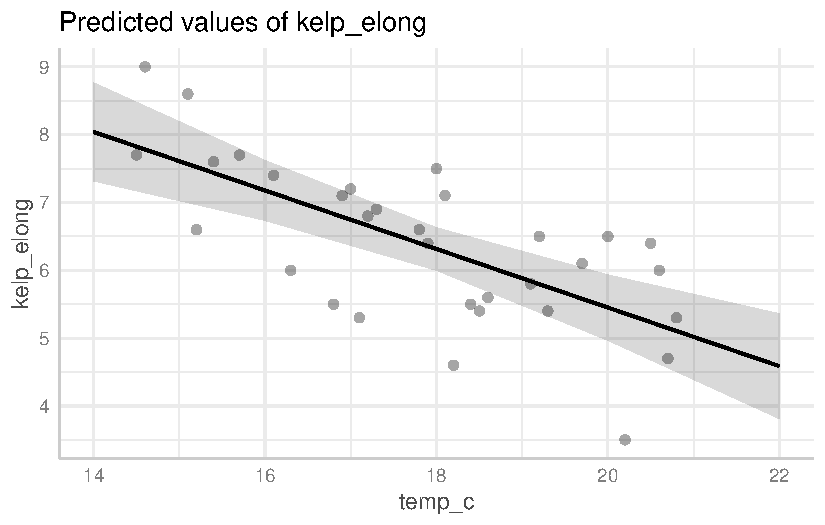
\includegraphics[keepaspectratio]{homework-03_files/figure-pdf/predicted-values-of-kelp_elong-1.pdf}}

\begin{Shaded}
\begin{Highlighting}[]
\CommentTok{\# running test to determine strength of correlation}
\FunctionTok{cor.test}\NormalTok{(temp\_kelp}\SpecialCharTok{$}\NormalTok{temp\_c, temp\_kelp}\SpecialCharTok{$}\NormalTok{kelp\_elong, }\AttributeTok{method =} \StringTok{"pearson"}\NormalTok{) }\CommentTok{\# pearson\textquotesingle{}s method}
\end{Highlighting}
\end{Shaded}

\begin{verbatim}

    Pearson's product-moment correlation

data:  temp_kelp$temp_c and temp_kelp$kelp_elong
t = -5.189, df = 30, p-value = 1.366e-05
alternative hypothesis: true correlation is not equal to 0
95 percent confidence interval:
 -0.8359665 -0.4460157
sample estimates:
       cor 
-0.6877489 
\end{verbatim}

\subsection{d.~Communication results}\label{d.-communication-results}

To evaluate the strength of the relationship between temperature and
giant kelp frond elongation rate, I used a Pearson's correlation because
the variables were continuous, mostly linear, and normally distributed,
enabling me to use this measurement.

We found a strong negative relationship between temperature and giant
kelp frond elongation rate (Pearson's r = -0.7, t(30) = -5.2, p
\textless{} 0.01, \(\alpha\) = 0.05), where temperature significantly
predicted kep elongation rate. From our model coeffiecient estimates, we
found that for each 1 degree Celsius increase in temperature, kelp
elongation rate decreases 0.43 ± 0.08 cm/day.

\subsection{e. How to apply test
results}\label{e.-how-to-apply-test-results}

Given the results of the Pearson's correlation test performed, there is
generally a negative relationship between temperature and kelp
elongation rate. This means that as temperature increases, the
elongation and growth rate of these kelp fronds are decreasing 0.43 ±
0.08 cm/day for every degree Celsius increase. If the team desires to
maximize kelp frond elongation, maintaining a water temperature around
14°C would maintain a higher elongation rate overall, meaning colder
ocean environments are more productive.

\subsection{f.~Double check}\label{f.-double-check}

\begin{Shaded}
\begin{Highlighting}[]
\CommentTok{\# running test to determine strength of correlation}
\FunctionTok{cor.test}\NormalTok{(temp\_kelp}\SpecialCharTok{$}\NormalTok{temp\_c, temp\_kelp}\SpecialCharTok{$}\NormalTok{kelp\_elong, }\AttributeTok{method =} \StringTok{"spearman"}\NormalTok{) }\CommentTok{\# spearman method}
\end{Highlighting}
\end{Shaded}

\begin{verbatim}

    Spearman's rank correlation rho

data:  temp_kelp$temp_c and temp_kelp$kelp_elong
S = 9216.1, p-value = 1.29e-05
alternative hypothesis: true rho is not equal to 0
sample estimates:
       rho 
-0.6891684 
\end{verbatim}

Using a Pearson's versus a Spearman correlation would have made no
difference, as in both tests there is a strong negative relationship
temperature and kelp elongation rate and the null hypothesis would be
rejected (Spearman \(\rho\) = -0.7, S = 9216.1, p \textless{} 0.01,
\(\alpha\) = 0.05). While the outputs mean the same thing, the test
components differ since a Pearson's correlation test outputs correlation
coefficient (r), a one-sample t-test comparing r to 0, and a 95\%
confidence interval, while a Spearman correlation test outputs the
correlation coefficient (\(\rho\)), the sum of all squared rank
differences (S), and no confidence intervals. Additionally, within the
data, there are tied ranks which leads the p-value commuted to be
approximate instead of exact for a Spearman correlation.

\section{Problem 2}\label{problem-2}

\subsection{a. Updating my data}\label{a.-updating-my-data}

\begin{Shaded}
\begin{Highlighting}[]
\CommentTok{\# creating new data frame using \textasciigrave{}my\_data\textasciigrave{}}
\NormalTok{my\_hist }\OtherTok{\textless{}{-}}\NormalTok{ my\_data }\SpecialCharTok{|\textgreater{}} 
  \CommentTok{\# cleaning column names so that only lower case letters and underscores are used}
  \FunctionTok{clean\_names}\NormalTok{()}
\CommentTok{\# reordering levels according to the day of the week in chronological order}
\NormalTok{my\_hist}\SpecialCharTok{$}\NormalTok{days }\OtherTok{\textless{}{-}} \FunctionTok{factor}\NormalTok{(my\_hist}\SpecialCharTok{$}\NormalTok{days,}
       \AttributeTok{levels =} \FunctionTok{c}\NormalTok{(}\StringTok{"Monday"}\NormalTok{, }\StringTok{"Tuesday"}\NormalTok{, }\StringTok{"Wednesday"}\NormalTok{, }\StringTok{"Thursday"}\NormalTok{, }\StringTok{"Friday"}\NormalTok{))}

\CommentTok{\# creating new data frame using \textasciigrave{}class\_num\textasciigrave{}}
\NormalTok{class\_num }\OtherTok{\textless{}{-}}\NormalTok{ bike\_to\_class }\SpecialCharTok{|\textgreater{}} 
  \CommentTok{\# cleaning column names so that only lower case letters and underscores are used}
  \FunctionTok{clean\_names}\NormalTok{()}
\end{Highlighting}
\end{Shaded}

\begin{Shaded}
\begin{Highlighting}[]
\CommentTok{\#base layer: ggplot}
\FunctionTok{ggplot}\NormalTok{(}\AttributeTok{data =}\NormalTok{ my\_hist,}
       \CommentTok{\# x{-}axis should be the day of the week and y{-}axis should be the time spent biking}
       \CommentTok{\# filling column color to differentiate days}
       \AttributeTok{mapping =} \FunctionTok{aes}\NormalTok{(}\AttributeTok{x =}\NormalTok{ days,}
                     \AttributeTok{y =}\NormalTok{ time\_spent\_biking\_min,}
                     \AttributeTok{fill =}\NormalTok{ days)) }\SpecialCharTok{+}
  \CommentTok{\# first layer: bar chart with height proportional to the values of the data}
  \FunctionTok{geom\_col}\NormalTok{(}\AttributeTok{width =} \FloatTok{0.5}\NormalTok{,}
           \CommentTok{\# color border line of bar black}
           \AttributeTok{color =} \StringTok{"black"}\NormalTok{,}
           \CommentTok{\# fill bin color pink}
           \AttributeTok{fill =} \StringTok{"pink"}\NormalTok{) }\SpecialCharTok{+}
  \CommentTok{\# relabeling x{-} and y{-}axes, adding title and subtitle}
  \FunctionTok{labs}\NormalTok{(}\AttributeTok{title =} \StringTok{"Comparison of total time spent biking throughout the week"}\NormalTok{,}
       \AttributeTok{subtitle =} \StringTok{"May 22, 2026"}\NormalTok{,}
       \AttributeTok{x =} \StringTok{"Day of the Week"}\NormalTok{,}
       \AttributeTok{y =} \StringTok{"Time Biking on Campus (min)"}\NormalTok{) }\SpecialCharTok{+}
  \CommentTok{\# changing theme of histogram}
  \FunctionTok{theme}\NormalTok{(}\AttributeTok{panel.background =} \FunctionTok{element\_blank}\NormalTok{()) }\SpecialCharTok{+}
  \CommentTok{\# removing legend}
  \FunctionTok{theme}\NormalTok{(}\AttributeTok{legend.position =} \StringTok{"none"}\NormalTok{)}
\end{Highlighting}
\end{Shaded}

\pandocbounded{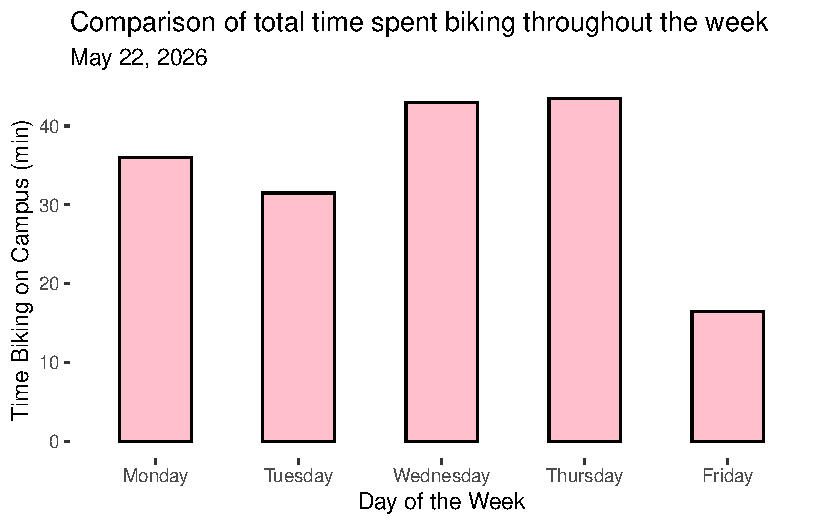
\includegraphics[keepaspectratio]{homework-03_files/figure-pdf/updated-personal-data-visuals-1.pdf}}

\begin{Shaded}
\begin{Highlighting}[]
\CommentTok{\# base layer: ggplot}
\FunctionTok{ggplot}\NormalTok{(}\AttributeTok{data =}\NormalTok{ class\_num,}
       \CommentTok{\# x{-}axis: number of classes per day}
       \CommentTok{\# y{-}axis: time spent biking (min)}
       \CommentTok{\# coloring by number of classes per day}
       \AttributeTok{mapping =} \FunctionTok{aes}\NormalTok{(}\AttributeTok{x =}\NormalTok{ number\_of\_classes\_per\_day,}
                     \AttributeTok{y =}\NormalTok{ time\_spent\_biking\_min,}
                     \AttributeTok{color =}\NormalTok{ number\_of\_classes\_per\_day)) }\SpecialCharTok{+}
  \CommentTok{\# first layer: jitter plot}
  \CommentTok{\# coloring data points by number of classes in custom coloration}
  \FunctionTok{geom\_jitter}\NormalTok{(}\AttributeTok{height =} \DecValTok{0}\NormalTok{,}
              \AttributeTok{width =} \FloatTok{0.1}\NormalTok{,}
              \FunctionTok{aes}\NormalTok{(}\AttributeTok{color =} \FunctionTok{factor}\NormalTok{(number\_of\_classes\_per\_day))) }\SpecialCharTok{+}
  \FunctionTok{scale\_color\_manual}\NormalTok{(}\AttributeTok{values =} \FunctionTok{c}\NormalTok{(}\StringTok{"1"} \OtherTok{=} \StringTok{"coral"}\NormalTok{,}
                                \StringTok{"2"} \OtherTok{=} \StringTok{"gold"}\NormalTok{,}
                                \StringTok{"3"} \OtherTok{=} \StringTok{"seagreen2"}\NormalTok{,}
                                \StringTok{"4"} \OtherTok{=} \StringTok{"royalblue3"}\NormalTok{)) }\SpecialCharTok{+}
  \CommentTok{\# relabeling x{-} and y{-}axes, adding a title and subtitle}
  \FunctionTok{labs}\NormalTok{(}\AttributeTok{title =} \StringTok{"Most biking occurs with one or two classes per day"}\NormalTok{,}
       \AttributeTok{subtitle =} \StringTok{"May 22, 2026"}\NormalTok{,}
       \AttributeTok{x =} \StringTok{"Number of Classes a Day (\#/day)"}\NormalTok{,}
       \AttributeTok{y =} \StringTok{"Time Spent Biking (min)"}\NormalTok{) }\SpecialCharTok{+}
  \CommentTok{\# changing theme to remove gridlines and any other visual clutter}
  \FunctionTok{theme}\NormalTok{(}\AttributeTok{panel.background =} \FunctionTok{element\_blank}\NormalTok{()) }\SpecialCharTok{+}
  \CommentTok{\# removing legend}
  \FunctionTok{theme}\NormalTok{(}\AttributeTok{legend.position =} \StringTok{"none"}\NormalTok{)}
\end{Highlighting}
\end{Shaded}

\pandocbounded{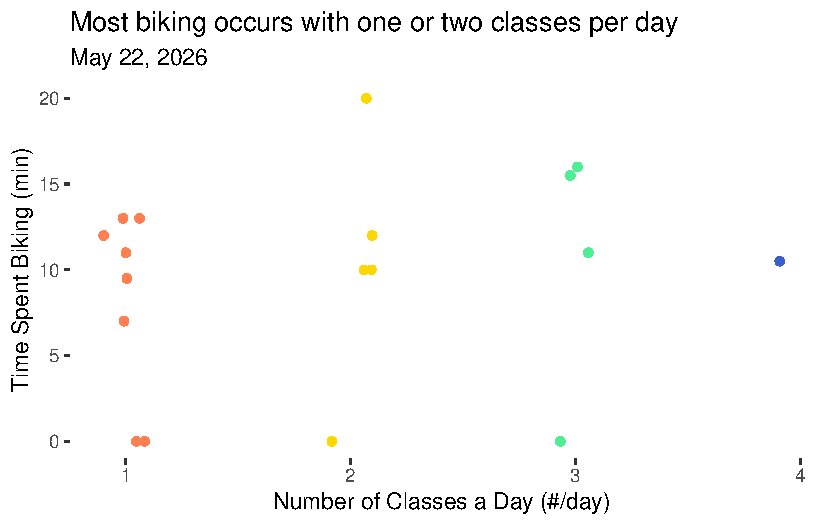
\includegraphics[keepaspectratio]{homework-03_files/figure-pdf/biking-classes-jitter-1.pdf}}

\subsection{b. Creating captions}\label{b.-creating-captions}

\textbf{Figure 1. The amount of time biking (min) differs across days of
the week.} The pink bins of the bar graph represent the cumulative
number of minutes spent biking on campus during that day of the week
over four weeks.

\textbf{Figure 2. The most occurrences of biking happen when there are
one or two classes had during the week.} Each colored point represents
measurements of time spent biking (min) across a different number of
classes (1-4). Colors differentiate the number of classes had during a
given day (coral: one class, yellow = two classes, green = three
classes, blue = 4 classes).

\section{Problem 3}\label{problem-3}

\subsection{a.}\label{a.}

As my data is about time spent biking on campus, I could focus on the
stress and anxiety of getting to class on time. The quicker I am biking
to my next destination is likely reflected by a faster bike ride, and so
the use of darker and more brooding colors could reflect this.
Additionally, the mental mania and obsession associated with academics,
timeliness, and fitting everything in could be represented with
purposefully disorienting, and maybe even lines of varying widths with
jagged angles. The idea is to create a visual affective piece that
evokes a feeling of stress and perpetual belatedness.

\subsection{b.}\label{b.}

\pandocbounded{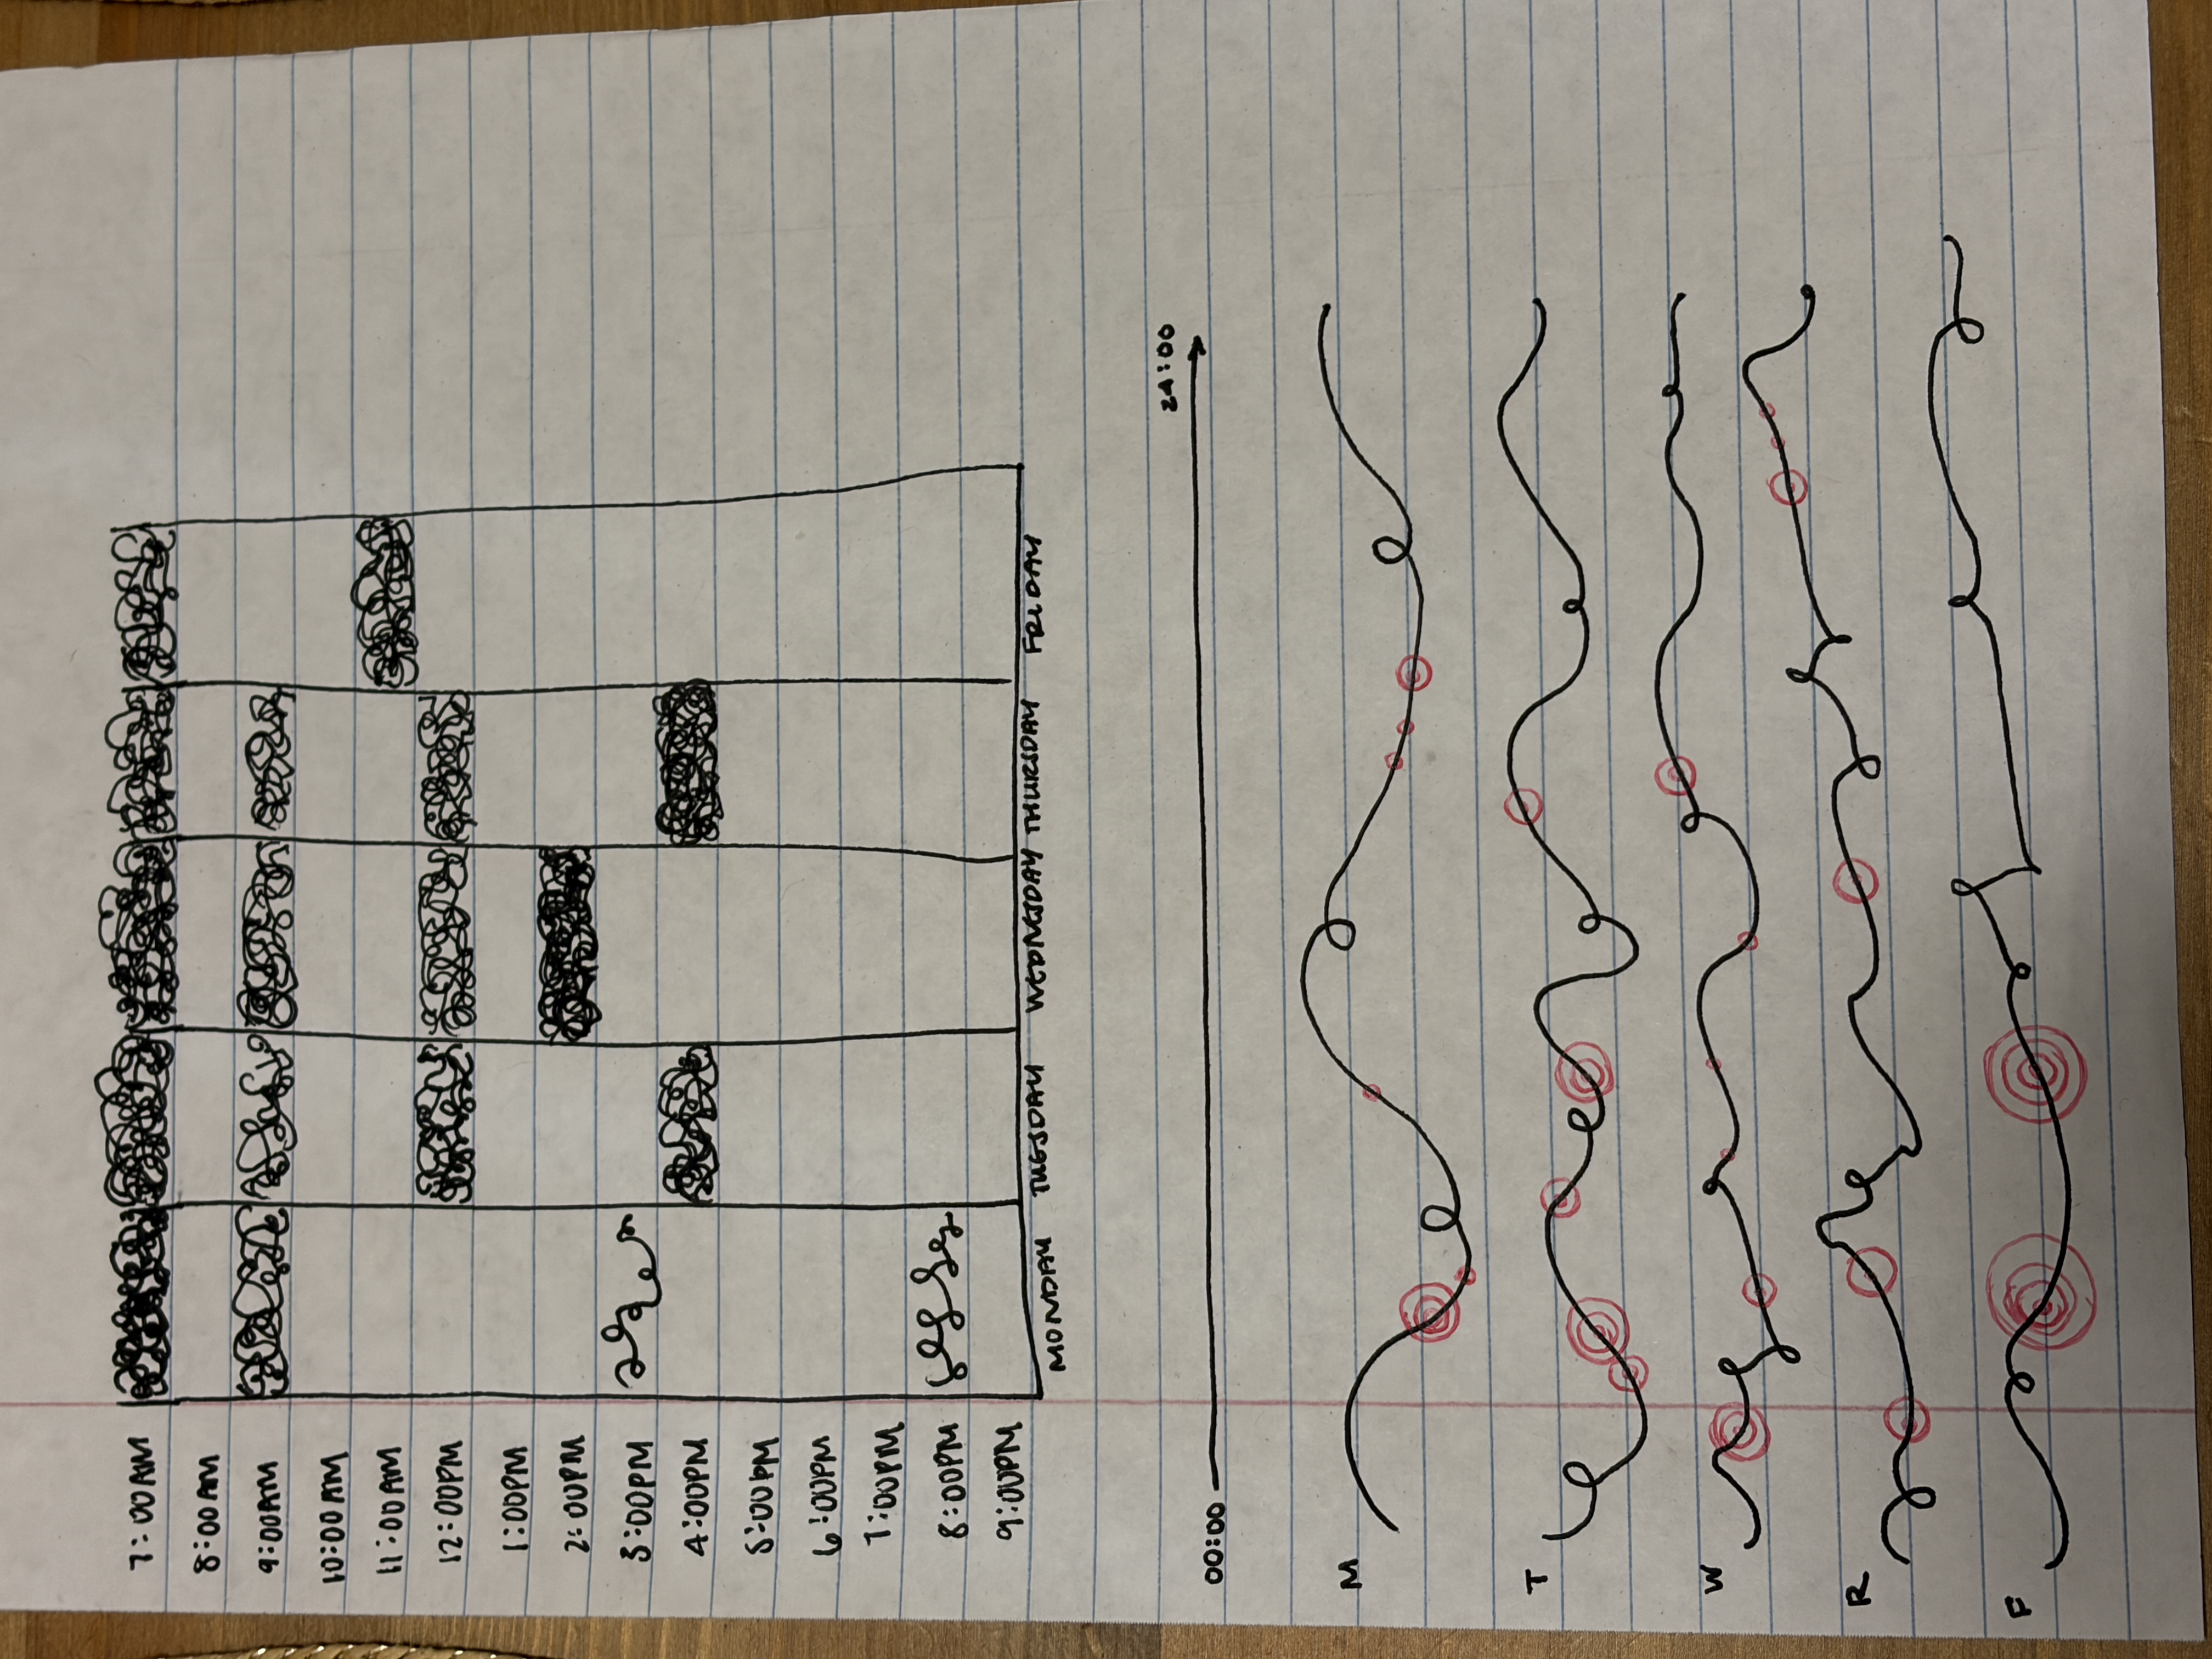
\includegraphics[keepaspectratio]{roughdrafts.png}}

\subsection{c.}\label{c.}

\pandocbounded{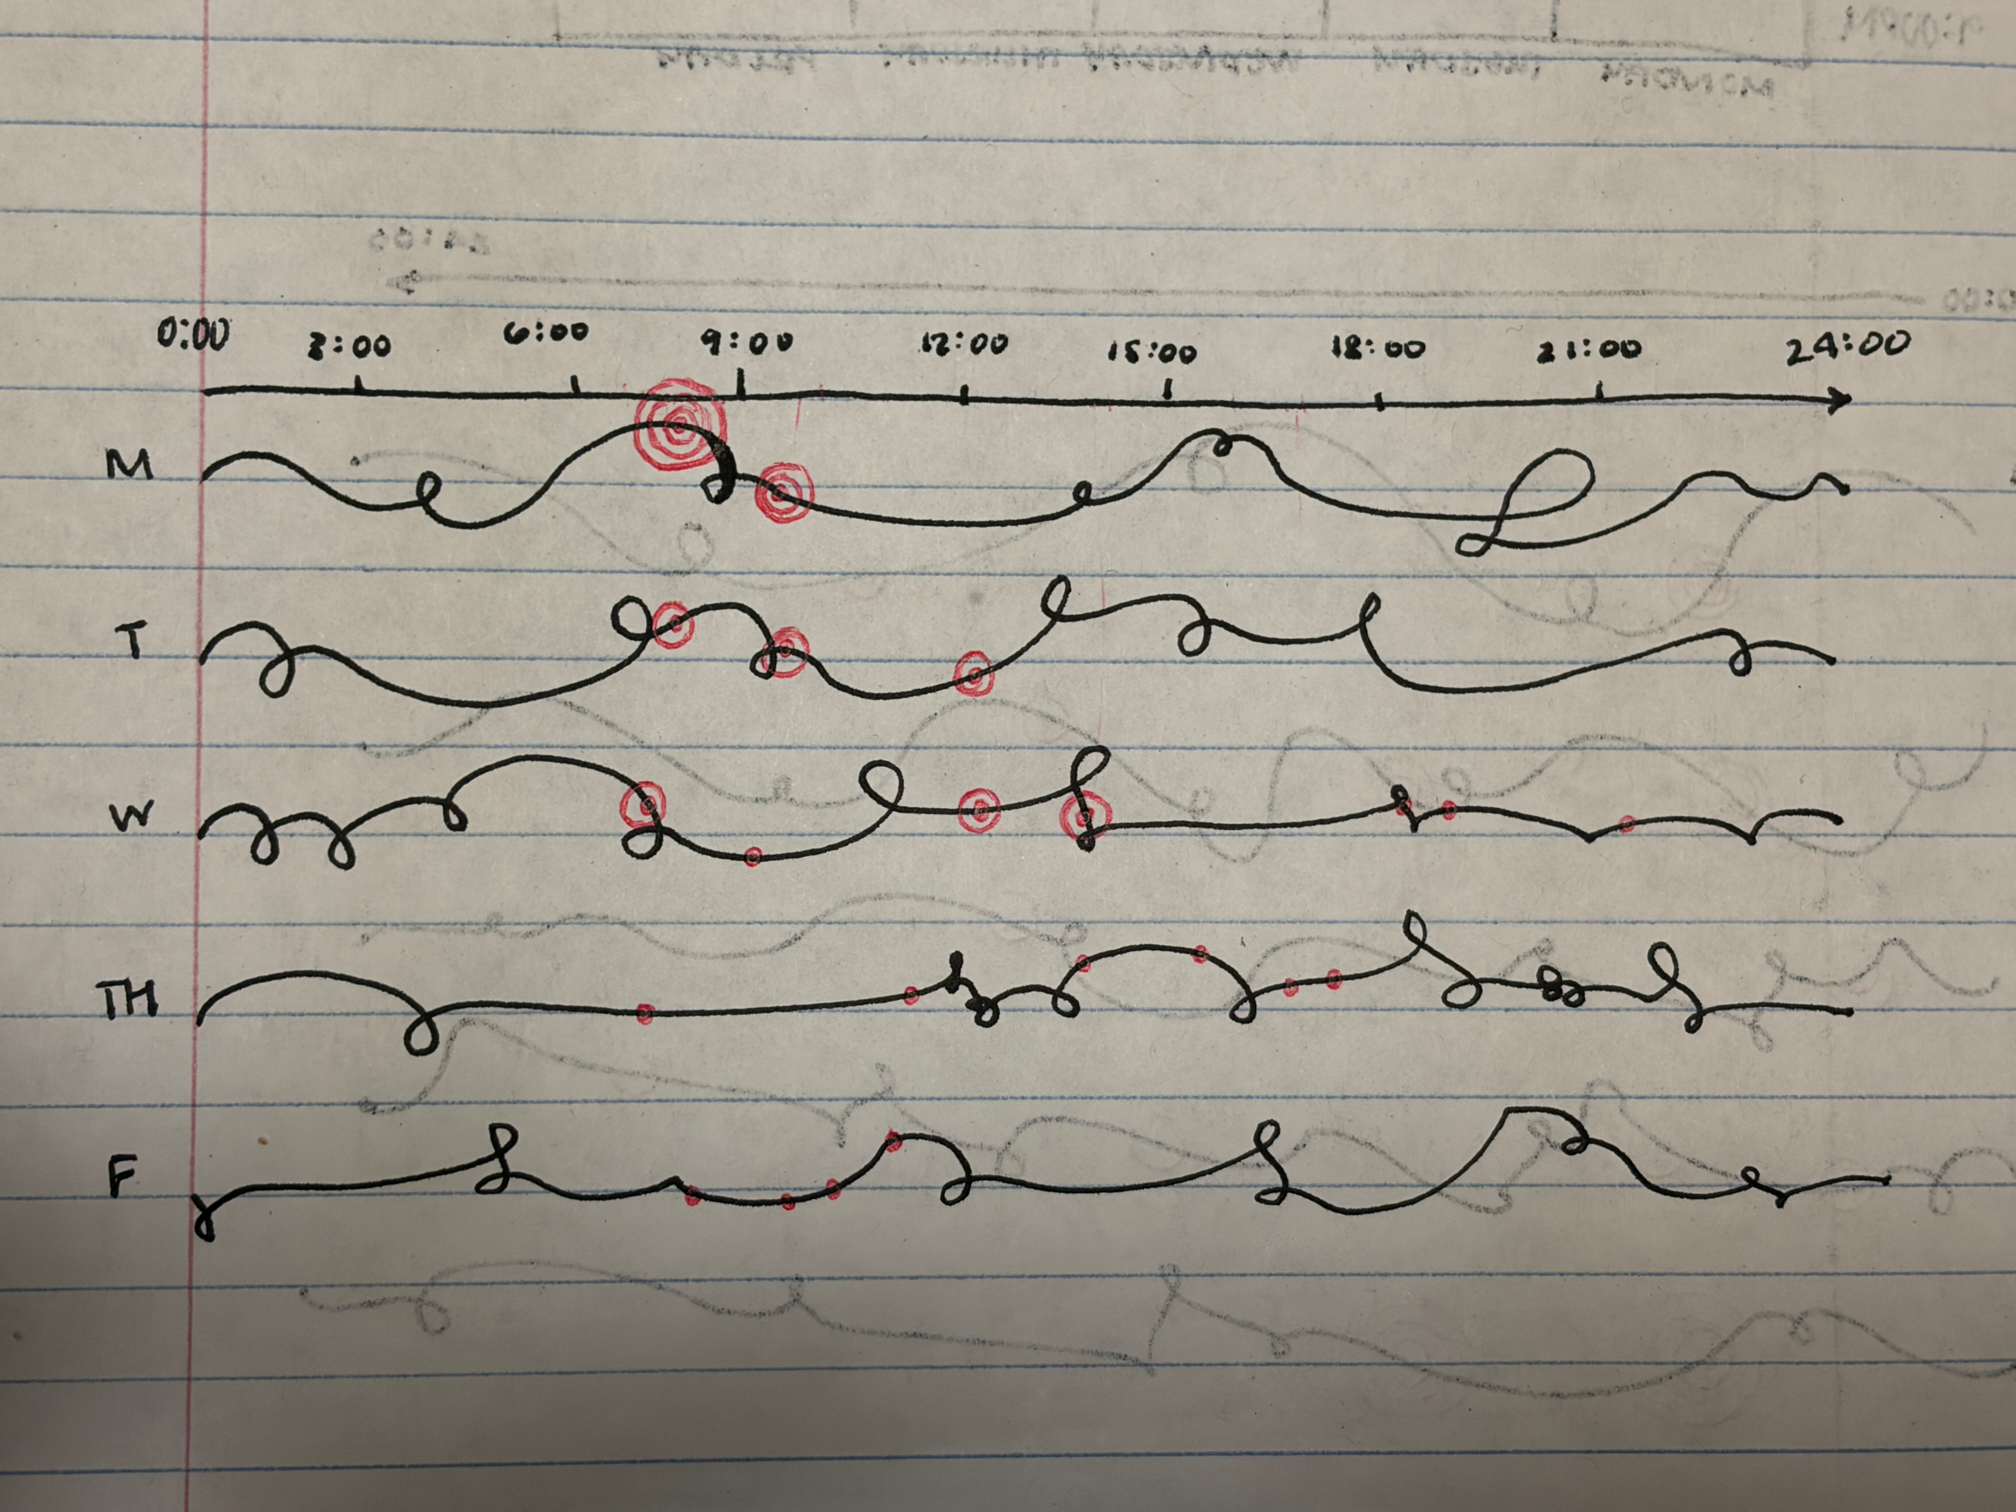
\includegraphics[keepaspectratio]{visudraft.png}}

\subsection{d.}\label{d.}

My piece shows the time of day over the weekdays in which I am biking to
class, with each additional circle representing my repetition of biking.
Each week was represented by a ``line in turmoil,'' where the stress of
the week and biking faster and faster from place to place was catching
up to me. The colors of black and red are also meant to work with color
theory such that the viewer is put at unease.

I was influenced to draw in this style by Stefanie Posavec and Giorgia
Lupi's ``Dear Data project,'' where weeks were shown and time was
recorded in wacky yet meaningful ways. I also found freehand drawing
with no real pattern to be perfect for the ``graph lines,'' as the
stress a student feels comes from all angles at times, and the mind is
constantly at unrest.

The form of my work in this rough draft is purely pen work, but in a
final draft I would like to add water color pens and a legend.

I was originally quite uninspired because biking doesn't seem to have
much emotion behind it. However, as I was thinking to my current state
of stress, my need to bike faster and faster from place to place, and
the lack of ``enough time'' during the day, I found there to be a large
mental health aspect inadvertently related to biking on school campuses.
When creating my work, I used the lines on my paper to create what I
call ``type-B precision,'' where each week begins at the beginning of
the red line, but goes bezerk following that, and I also used multiple
aspects of my personal data, implimenting it as Posavec and Lupi do so
well.

\subsection{e.}\label{e.}

\section{4.}\label{section}

\subsection{a. Revisit and summarize}\label{a.-revisit-and-summarize}

The paper that I selected in homework 1 uses a Mann-Whitney U test as
well as Kruskall Wallis test. However, I generally have been focusing on
the Mann-Whitney U component of this paper. In this case, a Mann-Whitney
U test addresses one of the main questions of the possible effects of
predation by finfish on sea urchin community structures, indicated by a
protected (isolated from fisherman and with abundant finfish) or
unprotected (not isolated from fisherman and with lower finfish
abundance) reef, rather than focusing on changes in urchin population
density variance due to normalization.

\pandocbounded{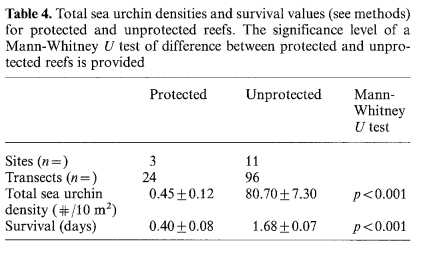
\includegraphics[keepaspectratio]{mann-whitney-u.png}}

\subsection{b. Visual clarity}\label{b.-visual-clarity}

Viewing the table I inserted above, the authors clearly visually
represented their statistics by placing the response variables in the
rows (total sea urchin density and survival) and the predictor variable
and its orders in the columns (reef protection - protected
vs.~unprotected), as well as whether the p-value is significant or not.
For each of these outcomes, a p-value will indicate whether there is a
significant difference between fisherman-protected and unprotected reefs
on fish shown in a clear manner. Additionally these outcomes each come
with a SE, which is some number above or below the calculation numbers.

\subsection{c.~Aesthetic clarity}\label{c.-aesthetic-clarity}

\pandocbounded{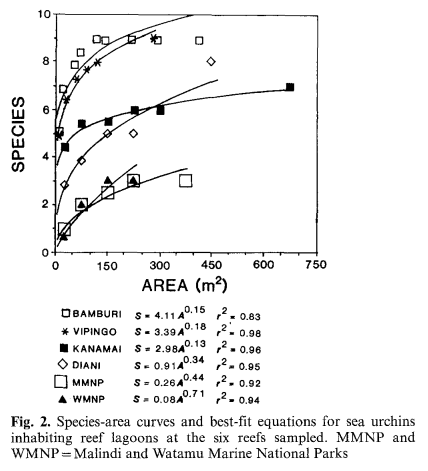
\includegraphics[keepaspectratio]{fig2-urchins.pdf}}

Within this figure, meant to show the differing groups of urchin species
depending on how large the area of observation is, there is generally a
low data:ink relationship. This is likely due to the overlapping slope
lines shown, and even with differing symbols for each reef lagoon, it is
still visually busy and a bit confusing. The most confusing aspects of
this graph are the outliers which overlap and cross over other lines,
furthering confusion of the viewer.

\subsection{d.~Recommendations}\label{d.-recommendations}

To make the figure 2 table more clear and visually appealing, there is
the potential to split the graph into multiple singe species-area curves
to reduce overlap confusion, omit the use of best-fit lines and connect
the individual points, or color each line and the corresponding points.
Splitting up the graphs into six smaller ones is definitely not the most
efficient and would take up more space, but would allow the comparison
of individual points to a greater extent. Connecting the points rather
than using a line of best fit would change each shape overall, but could
drastically increase precision and clarity of data. Lastly, and my
preferred solution, would be to pick individual colors for each reef
region, not changing the data or methods themselves, but bettering the
ability to pick out points to match with said region.




\end{document}
